\begin{definition}
    Sea $\boldsymbol{\Sigma}:D\subseteq\Rn{2}\to S\subseteq\Rn{3}$ una parametrizaci\'on inyectiva para todo $D$ en $S$. Se define el \textbf{borde} o \textbf{frontera} de $S$, y se lo nota $\partial S$, a la curva cerrada simple en $\Rn{3}$ tal que 
    \[
        \partial S=\boldsymbol{\Sigma}(\partial D).\finalmath
    \]
\end{definition}

\begin{obs} 
    Si $\partial D$ est\'a orientada de manera antihoraria, entonces $\boldsymbol{\Sigma}$ \textbf{induce} una orientaci\'on sobre $\partial S$. Adem\'as $\boldsymbol{\Sigma}$ \textbf{induce} una orientaci\'on sobre $S$.
\end{obs}

\begin{definition}
    Sea $D$ un conjunto conexo (en $\Rn{2}$ o en $\Rn{3}$). $D$ se llama \textbf{simplemente conexo} si toda curva cerrada simple $C\subset D$ es el borde de una regi\'on $R$ totalmente contenida en $D$.\final
\end{definition}

\begin{theorem}
    \textbf{Teorema de Green}. Sea $D\in\Rn{2}$ una regi\'on simplemente conexa y sea $\partial D$ la frontera de $D$, con orientaci\'on antihoraria. Y Sea $\mathbf{F}:D\to\Rn{2}$ de clase $C^1$. Entonces
    \[
        \oint_{\partial D}\mathbf{F}\cdot d\mathbf{s} = \iint_D \nabla\times\mathbf{F}\cdot d\mathbf{A}.\finalmath
    \]
\end{theorem}

\begin{obs} 
    Otra manera de enunciar el teorema de Green es usando un cambio en la notaci\'on vectorial. Pensando el producto escalar $\mathbf{F}\cdot d\mathbf{s}$ como $P\:dx+Q\:dy$, donde $\mathbf{F}=(P,Q)$ y sabiendo que el rotor en $\Rn{2}$ es la componente $z$ del rotor en $\Rn{3}$; reescribimos el teorema de Green como
\[
        \int_{\partial D}P\:dx+Q\:dy=\iint_D\left(\frac{\partial Q}{\partial x}-\frac{\partial P}{\partial y}\right).
\]
\end{obs}

\begin{obs}
    \textbf{Extensi\'on de Green.} El teorema de Green es aplicable a regiones a\'un m\'as generales que simplemente conexas. De hecho, a cualquier regi\'on en $\Rn{2}$ cuya frontera se pueda descomponer en un n\'umero finito de curvas cerradas simples orientadas se le puede aplicar el teorema de Green. La idea es ``recorrer" dicha frontera pasando por todas las curvas que la confroman.
\end{obs}

\begin{center}
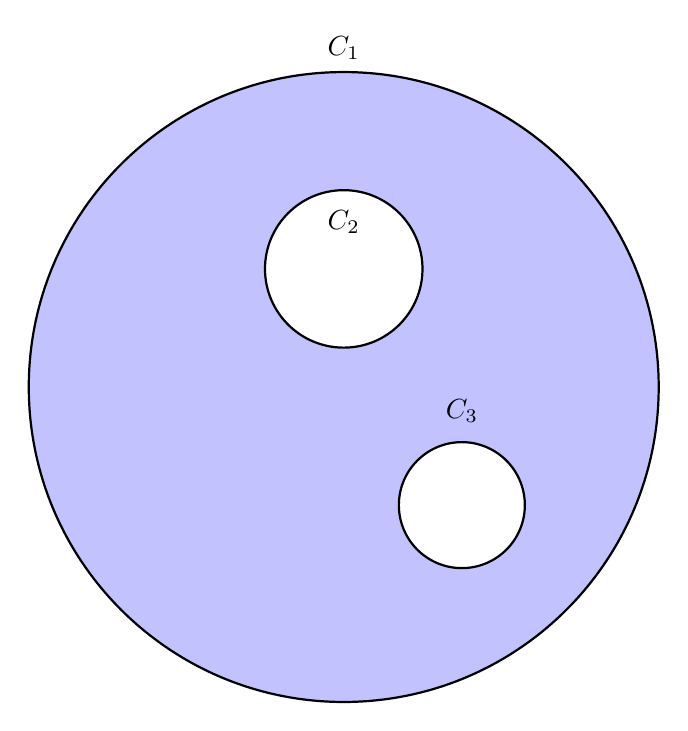
\begin{tikzpicture}
    % Define the exterior boundary
    \draw[thick, fill=blue!60!white!40] (0,0) circle (4);

    % Define the inner boundaries
    \draw[thick, fill=white] (0,1.5) circle (1);
    \draw[thick, fill=white] (1.5,-1.5) circle (0.8);

    % % Draw arrows for the outer boundary
    \ARW[thick,red,<-]{0, 0, 0, 347};

    % Label the regions
    \node at (0,4.3) {$C_1$};
    \node at (0,2.1) {$C_2$};
    \node at (1.5,-0.3) {$C_3$};

\end{tikzpicture}
\end{center}
\textcolor{red}{falta poner las flechas que indican la orientacion}

\begin{theorem}
\textbf{Teorema de la divergencia en el plano}. Sea $D\subset\Rn{2}$ una regi\'on donde valga Green y sea $\partial D$ su frontera. Denotaremos por $\mathbf{n}$ el versor unitario normal a $\partial D$ en todo punto. Si $\boldsymbol{\sigma}:[a,b]\to\Rn{2},\;\boldsymbol{\sigma}(t)=(x(t),y(t))$ es una parametrizaci\'on orientada de manera positiva de $\partial D$, $\mathbf{n}$ est\'a dado por 
\[
    \mathbf{n}=\frac{(y'(t),-x'(t))}{\sqrt{[x'(t)]^2+[y'(t)]^2}}.
\]
Sea $\mathbf{F}$ un campo vectorial $C^1$ en $D$. Entonces
\[
    \int_{\partial D}\mathbf{F}\cdot\mathbf{n}\:ds=\iint\nabla\cdot\mathbf{F}\:dA.\finalmath
\]
\end{theorem}

\begin{theorem}
\textbf{Teorema de Stokes}. Sea $S\subset\Rn{3}$ una superficie parametrizada por $\boldsymbol{\Sigma}:D\subset\Rn{3}to S$, donde las orientaciones de $S$ y $\partial S$ fueron inducidas por $\boldsymbol{\Sigma}$. Si $\mathbf{F}:$ es un campo vectorial $C^1$ en $S$. Entonces
\[
    \oint_{\partial S}\mathbf{F}\cdot d\mathbf{s}=\iint_S\nabla\times\mathbf{F}\cdot d\mathbf{A}.\finalmath
\]
\end{theorem}

\begin{theorem}
\textbf{Teorema de la divergencia o de Gauss}. Sea $S\subset\Rn{3}$ una superficie que encierra un volumen $\Omega$ orientada de manera exterior, esto es $S=\partial \Omega$. Sea $\mathbf{F}:\Omega\to\Rn{3}$ un campo vectorial clase $C^1$, entonces
\[
    \oiint_{\partial \Omega}\mathbf{F}\cdot d\mathbf{S}=\iiint_{\Omega}\nabla\cdot\mathbf{F}\:dV.\finalmath
\]
\end{theorem}